\documentclass[a4paper,11pt]{jsarticle}

% 数式
\usepackage{amsmath,amsfonts}
\usepackage{amsthm}
\usepackage{bm}
\usepackage{mathtools}
\usepackage{amssymb}

% 表
\usepackage[utf8]{inputenc}
\usepackage{diagbox} % 斜線付きセルを作成するために必要
\usepackage{booktabs} % 表の罫線を美しくするために必要
\usepackage{hhline} % 水平罫線を制御するために必要

% 画像
\usepackage[dvipdfmx]{graphicx}
\usepackage{ascmac}
\usepackage{physics}
\usepackage{float} % 追加

% 図
\usepackage[dvipdfmx]{graphicx}
\usepackage{tikz} %図を描く
\usetikzlibrary{positioning, intersections, calc, arrows.meta,math} %tikzのlibrary

% ハイパーリンク
\usepackage[dvipdfm,
  colorlinks=false,
  bookmarks=true,
  bookmarksnumbered=false,
  pdfborder={0 0 0},
  bookmarkstype=toc]{hyperref}

% 式番号を章ごとにリセット
\numberwithin{equation}{section}

\begin{document}

\title{Majorization}
\author{大上由人}
\date{\today}
\maketitle

\tableofcontents
\newpage

\section{リソース理論と確率熱力学の位置づけ}
非平衡状態の熱力学第二法則を考えるときに、これまで二つのアプローチがとられてきた。\\
\subsection{確率熱力学的アプローチ}
確率熱力学においては、仕事の揺らぎを許した系を考え、ゆらぎの定理の系として、エントロピー生成の熱力学第二法則が導かれる。\\

\subsection{リソース理論的アプローチ}
リソース理論においては、外部からの仕事は完全に制御されたものとし、系の状態を変化させるために必要なリソースを考える。\\
\begin{itembox}[l]{\textbf{Def:free state/free operation}}
    何のコストもなしに得られる状態をfree state、何のコストもなしに行える操作をfree operationという。
\end{itembox}
熱力学リソース理論においては、熱浴に接触した系の状態や遷移を考える。以下が、free state/free operation/resourceの対応である。\\
\begin{itemize}
    \item free state:熱平衡状態
    \item free operation:緩和過程(GPM)
    \item resource:仕事/非平衡状態
\end{itemize}

さらに、monotoneと呼ばれる概念も重要である。\\
\begin{itembox}[l]{\textbf{Def:monotone}}
    free operationに対して、単調に変化する量をmonotoneという。とくに、ある操作が可能かどうかの必要十分条件を与えるmonotoneをcomplete monotoneという。
\end{itembox}
我々の目的は、complete monotoneを見つけて、遷移可能性を評価することである。\\

\textbf{ex:従来の熱力学}\\
従来の熱力学におけるresource、free state、free operation、(complete) monotoneは以下のように対応する。\\
\begin{itemize}
    \item resource:仕事
    \item free state:熱平衡状態
    \item free operation:断熱操作
    \item (complete) monotone:エントロピー
\end{itemize}

\subsection{確率熱力学とリソース理論の関係}
両者は、出所やset upが異なるが、マクロ極限をとると、同じ第二法則が導かれる。\\

\newpage
\section{古典的エントロピー及びダイバージェンス}
\subsection{古典的状態及び系}
必要な量を定義する。\\
\begin{itembox}[l]{\textbf{Def:状態を表す確率分布}}
    古典的系における状態は確率分布
    \begin{equation}
        p = (p_1, p_2, \cdots, p_d)^{\top}
    \end{equation}
    で表される。ここで、$p_i \geq 0$かつ$\sum_{i=1}^{d}p_i = 1$である。
    また、d次元の確率分布全体の集合を、$\mathcal{P}_d$と表す。\\
    また、その集合に属する一様分布を、
    \begin{equation}
        u = \left(\frac{1}{d}, \frac{1}{d}, \cdots, \frac{1}{d}\right)^{\top}
    \end{equation}
    と表す。\\
    また、異なる確率分布の積を、
    \begin{equation}
        p \otimes q \in \mathcal{P}_{dd'} \quad p \in \mathcal{P}_d, q \in \mathcal{P}_{d'}
    \end{equation}
    と表し、とくに、同じ確率分布の累乗を、
    \begin{equation}
        p^{\otimes n} \in \mathcal{P}_{d^n} \quad p \in \mathcal{P}_d
    \end{equation}
    と表す。
\end{itembox}

\begin{itembox}[l]{\textbf{Def:Supp}}
    確率分布$p ={p_i}_i \in \mathcal{P}_d$に対して、pの台を、
    \begin{equation}
        \text{supp}(p) = \{i \in [d] | p_i > 0\} \subset \{1, 2, \cdots, d\}
    \end{equation}
    と表す。また、
    \begin{equation}
        \text{rank}(p) = |\text{supp}(p)|
    \end{equation}
    を、pのランクという。とくに、$\text{rank}(p) = d$のとき、pはフルランクであるという。
\end{itembox}
要するに、確率が0でないようなインデックスの集合を台と呼び、その要素数をランクと呼ぶ。\\

\begin{itembox}[l]{\textbf{Def:確率遷移行列}}
    古典的な確率分布の時間発展は、確率遷移行列$T$を用いて以下のように表される。
    \begin{equation}
        p_i ' = \sum_{j=1} T_{ij}p_j 
    \end{equation}
\end{itembox}

\begin{itembox}[l]{\textbf{Prop:確率遷移行列の性質}}
    確率遷移行列$T$は以下の性質を持つ。
    \begin{equation}
        \sum_{i=1}^{d}T_{ij} = 1
    \end{equation}
\end{itembox}
\textbf{Prf}\\
略(確率の規格化を利用する。)\hfill \qedsymbol\\

\begin{itembox}[l]{\textbf{Def:二重確率遷移行列}}
    確率遷移行列$T$が、
    \begin{equation}
        \sum_{j=1} T_{ij} = 1
    \end{equation}
    をみたすとき、二重確率遷移行列という。
\end{itembox}
\begin{itembox}[l]{\textbf{Prop:二重確率遷移行列の特徴づけ}}
    以下の二つは同値である。
    \begin{enumerate}
        \item Tは二重確率遷移行列である。
        \item 一様分布uはTに対して不変である。すなわち、$u=Tu$である。
    \end{enumerate}
\end{itembox}
\textbf{Prf}\\
\begin{align}
    p_i ' &= \sum_{j=1} T_{ij}u_j\\
    &= \frac{1}{d}\sum_{j=1}^{d}T_{ij}\\
    &= \frac{1}{d}\cdot d\\
    &= 1
\end{align}
であることからわかる。\\

\begin{itembox}[l]{\textbf{Def:トレース距離}}
    二つの確率分布$p, q$のトレース距離は、
    \begin{equation}
        D(p, q) = \frac{1}{2}\sum_{i=1}^{d}|p_i - q_i|
    \end{equation}
    で定義される。
\end{itembox}
\begin{itembox}[l]{\textbf{Prop:トレース距離の性質}}
    トレース距離は、$T$に対して非増加である。すなわち、
    \begin{equation}
        D(p,q) \geq D(Tp, Tq)
    \end{equation}
    が成り立つ。
\end{itembox}
\textbf{Prf}\\
後により一般の証明をするため、ここでは省略する。\\

\subsection{シャノンエントロピー及びKLダイバージェンス}
\begin{itembox}[l]{\textbf{Def:シャノンエントロピー}}
    確率分布$p \in \mathcal{P}_d$のシャノンエントロピーは、
    \begin{equation}
        S_1(p) = -\sum_{i=1}^{d}p_i\log p_i
    \end{equation}
    で定義される。
\end{itembox}
\begin{itembox}[l]{\textbf{Def:KLダイバージェンス}}
    二つの確率分布$p, q \in \mathcal{P}_d$のKLダイバージェンスは、
    \begin{equation}
        S_1(p||q) = \sum_{i=1}^{d}p_i\log\frac{p_i}{q_i}
    \end{equation}
    で定義される。ただし、$\text{supp}(p) \subset \text{supp}(q)$でないときは、$S_1(p||q) = \infty$とする。
\end{itembox}
このとき、エントロピーとKLダイバージェンスの関係がわかる。
\begin{itembox}[l]{\textbf{Prop:エントロピーとKLダイバージェンスの関係}}
    任意の$p, q \in \mathcal{P}_d$に対して、
    \begin{equation}
        S_1(p) = \log(d) - S_1(p||u)
    \end{equation}
\end{itembox}
\textbf{Prf}\\
\begin{align}
    S_1(p||u) &= \sum_{i=1}^{d}p_i\log\frac{p_i}{\frac{1}{d}}\\
    &= \sum_{i=1}^{d}p_i\log dp_i\\
    &= \sum_{i=1}^{d}p_i\log d + \sum_{i=1}^{d}p_i\log p_i\\
    &= \log d - S_1(p)
\end{align}
であることからわかる。\hfill \qedsymbol\\
これより、$S_1(p) \leq \log d$であることがわかる。\\
このとき、KLダイバージェンスのテイラー展開は、$\log \frac{1}{1-x}$のテイラー展開を用いて\footnote{$x+\frac{x^2}{2}+\cdots $}、以下のようになる。
\begin{align}
    S_1(p||p-\Delta p) &= \frac{1}{2}\sum_i \frac{(\Delta p_i)^2}{p_i} + O(\Delta p^3)\\
\end{align}
ここで、$\sum_i \Delta p_i = 0$を用いている。\\

\begin{itembox}[l]{\textbf{Prop:KLダイバージェンスの単調性}}
    KLダイバージェンスは、$p' = Tp$および$q' = Tq$に対して、
    \begin{equation}
        S_1(p||q) \geq S_1(p'||q')
    \end{equation}
    が成り立つ。
\end{itembox}
\textbf{Prf}\\
後に一般に示す。\\

注意されたいこととして、KLダイバージェンスの単調性の逆はいえない。すなわち、単調性を満たすが、$p' = Tp$および$q' = Tq$を満たすような$T$が存在しない場合がある。\\

次に、二重確率遷移行列について考える。このとき、KLダイバージェンスの単調性と、
\begin{equation}
    S_1(p) \leq S_1(Tp)
\end{equation}
が成り立つ。\\
すなわち、二重確率遷移行列による時間発展は、エントロピーを増加させる。\\

\begin{itembox}[l]{\textbf{Def:相互情報量}}
    二つの確率分布$p, q \in \mathcal{P}_d$の相互情報量は、
    \begin{equation}
        I_1 (p_{AB})_{A:B} = S_1 (p_A) + S_1 (p_B) - S_1 (p_{AB}) = S_1(p_{AB}||p_A \otimes p_B) \geq 0
    \end{equation}
    で定義される。
\end{itembox}
この量は、AとBの相関を表す量である。\\
\begin{itembox}[l]{\textbf{Prop:相互情報量の性質}}
    任意の$p, q \in \mathcal{P}_d$に対して、
    \begin{equation}
        I_1(p_{AB})_{A:B} =0 \Leftrightarrow p_{AB} = p_A \otimes p_B
    \end{equation}
    が成り立つ。また、KLダイバージェンスの単調性から、
    \begin{equation}
        I_1(p_{AB})_{A:B} \geq I_1(T_A \otimes T_B p_{AB})_{A:B}
    \end{equation}
    が成り立つ。ただし、$T_A \otimes T_B$は、各A,Bに独立に作用する確率遷移行列である。\\
    
\end{itembox}
\textbf{Prf}\\
略(過去のゼミ資料を参考せよ)\hfill \qedsymbol\\

\subsection{Rényiエントロピー及びダイバージェンス}
シャノンエントロピーを包含する概念として、Rényiエントロピーがある。\\
\begin{itembox}[l]{\textbf{Def:Rényiエントロピー}}
    確率分布$p \in \mathcal{P}_d$のRényiエントロピーは、$0 \leq \alpha \leq \infty$、$p \in \mathcal{P}_d$に対して、
    \begin{equation}
        S_{\alpha}(p) = \frac{1}{1-\alpha}\log(\sum_{i=1}^{d}p_i^{\alpha})
    \end{equation}
    で定義される。
\end{itembox}
また、ダイバージェンスについても、Rényiダイバージェンスがある。\\
\begin{itembox}[l]{\textbf{Def:Rényiダイバージェンス}}
    二つの確率分布$p, q \in \mathcal{P}_d$のRényiダイバージェンスは、$0 \leq \alpha \leq \infty$、$p \in \mathcal{P}_d$に対して、
    \begin{equation}
        S_{\alpha}(p||q) = \frac{1}{\alpha - 1}\log(\sum_{i=1}^{d}p_i^{\alpha}q_i^{1-\alpha})
    \end{equation}
    で定義される。ただし、$\text{supp}(p) \subset \text{supp}(q)$でないときは、$S_{\alpha}(p||q) = \infty$とする。
\end{itembox}
これらの量が、たしかにシャノンエントロピーとKLダイバージェンスを包含していることを示す。\\
\begin{itembox}[l]{\textbf{Prop:Rényiエントロピーとシャノンエントロピーの関係}}
    Rényi-1エントロピーは、シャノンエントロピーに一致する。すなわち、
    \begin{equation}
        S_1(p) = S_{\alpha}(p)|_{\alpha = 1}
    \end{equation}
    が成り立つ。
\end{itembox}
\textbf{Prf}\\
\begin{align}
    S_{\alpha}(p)|_{\alpha = 1} &= -lim_{\alpha \to 1}\frac{1}{1-\alpha}\log(\sum_{i=1}^{d}p_i^{\alpha})\\
    &= -\frac{d}{d\alpha}\log(\sum_{i=1}^{d}p_i^{\alpha})|_{\alpha = 1}\\
    &= -\frac{\sum_{i=1}^{d}p_i\log p_i}{\sum_{i=1}^{d}p_i}\\
    &= -\sum_{i=1}^{d}p_i\log p_i\\
    &= S_1(p)
\end{align}
であることからわかる。\hfill \qedsymbol\\

\begin{itembox}[l]{\textbf{Prop:Rényiダイバージェンスとダイバージェンスの関係}}
    Rényi-1ダイバージェンスは、KLダイバージェンスに一致する。すなわち、
    \begin{equation}
        S_{\alpha}(p||q)|_{\alpha = 1} = S_1(p||q)
    \end{equation}
    が成り立つ。
\end{itembox}
\textbf{Prf}\\
\begin{align}
    S_{\alpha}(p||q)|_{\alpha = 1} &= lim_{\alpha \to 1}\frac{1}{\alpha - 1}\log(\sum_{i=1}^{d}p_i^{\alpha}q_i^{1-\alpha})\\
    &= \frac{d}{d\alpha}\log(\sum_{i=1}^{d}p_i^{\alpha}q_i^{1-\alpha})|_{\alpha = 1}\\
    &= \frac{\sum_{i=1}^{d}q_i(p_i/q_i)^{\alpha}\log (p_i/q_i)}{\sum_{i=1}^{d}p_i^{\alpha}q_i^{1-\alpha}}|_{\alpha = 1}\\%TODOここの計算後で確認する。
    &= \sum_{i=1}^{d}p_i\log\frac{p_i}{q_i}\\
    &= S_1(p||q)
\end{align}
であることからわかる。\hfill \qedsymbol\\

また、$\alpha =0,\infty$の場合は重要らしいので、以下で確認する。
\begin{itembox}[l]{\textbf{Prop:Rényiエントロピー/ダイバージェンスの極限}}
    Rényi-0エントロピーは、
    \begin{equation}
        S_0(p) = \log (\text{rank}(p))
    \end{equation}
    で定義される。また、Rényi-$\infty$エントロピーは、
    \begin{equation}
        S_{\infty}(p) = -(\log \max_{i}p_i)
    \end{equation}
    で定義される。また、Rényi-0ダイバージェンスは、
    \begin{equation}
        S_0(p||q) = -\log (\sum_{i:p_i > 0}q_i)
    \end{equation}
    で定義される。また、Rényi-$\infty$ダイバージェンスは、
    \begin{equation}
        S_{\infty}(p||q) = \log (\max_{i}\frac{p_i}{q_i})
    \end{equation}
    で定義される。
\end{itembox}
\textbf{Prf}\\
%TODO後で示す。\alpha=0については自明\\

\begin{itembox}[l]{\textbf{Prop:RényiエントロピーとKLダイバージェンスの関係}}
    任意の$p, q \in \mathcal{P}_d$に対して、
    \begin{equation}
        S_{\alpha}(p) = \frac{1}{1-\alpha}\log d - S_{\alpha}(p||u)
    \end{equation}
    が成り立つ。
\end{itembox}

以下、Rényiダイバージェンスについての性質を示す。\\
\begin{itembox}[l]{\textbf{Prop:Rényiダイバージェンスの非負性}}
    任意の$p, q \in \mathcal{P}_d$に対して、
    \begin{equation}
        S_{\alpha}(p||q) \geq 0
    \end{equation}
    が成り立つ。また、$0 < \alpha \leq  \infty$に対して、
    \begin{equation}
        S_{\alpha}(p||q) =0 \Leftrightarrow p = q
    \end{equation}
    であり、また、$\alpha =0$のとき、
    \begin{equation}
        S_{0}(p||q) = 0 \Leftrightarrow \text{supp}(p) \subset \text{supp}(q)
    \end{equation}
    が成り立つ。
\end{itembox}

\begin{itembox}[l]{\textbf{Prop:Rényiダイバージェンスの単調性}}
    任意の$p' = Tp, q' = Tq \in \mathcal{P}_d$に対して、
    \begin{equation}
        S_{\alpha}(p||q) \geq S_{\alpha}(p'||q')
    \end{equation}
    が成り立つ。また、二重確率遷移行列に対して、
    \begin{equation}
        S_{\alpha}(p) \leq S_{\alpha}(Tp)
    \end{equation}
    が成り立つ。
\end{itembox}

\begin{itembox}[l]{\textbf{Prop:Rényiダイバージェンスの単調性(2)}}
    $\alpha \leq \alpha' $に対して、
    \begin{equation}
        S_{\alpha}(p||q) \leq S_{\alpha'}(p||q)
    \end{equation}
    が成り立ち、また、
    \begin{equation}
        S_{\alpha}(p) \geq S_{\alpha'}(p)
    \end{equation}
    が成り立つ。
\end{itembox}

\begin{itembox}[l]{\textbf{Lem:}}
    fを下に凸な関数であるとし、$p,q,p',q' \in \mathbb{R}^d$がすべて正であるとする。
    もし、$p' = Tp, q' = Tq$であるとき、
    \begin{equation}
        \sum_{i=1}^{d} q_i'f\left(\frac{p_i'}{q_i'}\right) \leq \sum_{i=1}^{d} q_i f\left(\frac{p_i}{q_i}\right)
    \end{equation}
    が成り立つ。
\end{itembox}
\textbf{Prf}\\
Jensenの不等式より、
\begin{equation}
    \sum_{j=1}^{d}q_j'f\left(\frac{p_j'}{q_j'}\right) \leq \sum_{j=1}^{d}\sum_{i=1}^{d}\frac{T_{ji}q_i}{q_j'}f\left(\frac{p_i}{q_i}\right)=\sum_{i=1}^{d}q_i f\left(\frac{p_i}{q_i}\right)
\end{equation}
である。\hfill \qedsymbol\\
ここで、$p,q \in \mathcal{P}_d$として、$f(x)=x\log x$とすると、
\begin{equation}
    S_1 (p||q) \geq S_1 (p'||q')
\end{equation}
が成り立つ。これは、KLダイバージェンスの単調性を示している。\\

\textbf{Prf:(Rényiダイバージェンスの非負性)}\\
$f_{\alpha}(x) = x^{\alpha}$とすると、$1<\alpha \leq \infty$に対して、$f_{\alpha}(x)$は下に凸な関数である。\\
Jensenの不等式より
\begin{equation}
    \sum_{i=1}^{d}q_i f(\frac{p_i}{q_i}) \geq f(\sum_{i=1}^{d}q_i \frac{p_i}{q_i}) = f(1) = 0
\end{equation}
である。両辺対数をとることにより、
\begin{equation}
    \log(\sum_{i=1}^{d}q_i \frac{p_i}{q_i}) \geq 0
\end{equation}
である。これを両辺$\frac{1}{\alpha - 1}$かけることにより、
\begin{equation}
    \frac{1}{\alpha - 1}\log(\sum_{i=1}^{d}q_i \frac{p_i}{q_i}) \geq 0
\end{equation}
である。したがって、
\begin{equation}
    S_{\alpha}(p||q) \geq 0
\end{equation}
である。また、$0 < \alpha <1$のときは、上のJensenの不等式で不等号が逆になり、$\frac{1}{\alpha-1}$をかけるときにもう一度符号が逆になることに注意して、同様に示すことができる。\\
$\alpha =0,1,\infty$の場合は、それぞれの定義から自明である。\\  
\hfill \qedsymbol\\

\textbf{Prf:(Rényiダイバージェンスの単調性)}\\
$1<\alpha <\infty$のとき、Lemで、$f(x) = x^{\alpha}$として示した不等式を用いると、
\begin{equation}
    \sum_{i=1}^{d}q_i'\frac{p_i'^{\alpha}}{q_i'^{\alpha}} \leq \sum_{i=1}^{d}q_i\frac{p_i^{\alpha}}{q_i^{\alpha}}
\end{equation}
である。これの両辺対数をとることにより、
\begin{equation}
    \log(\sum_{i=1}^{d}p_i'^{\alpha}q_i^{1-\alpha}) \leq \log(\sum_{i=1}^{d}p_i^{\alpha}q_i^{1-\alpha})
\end{equation}
である。したがって、
\begin{equation}
    \frac{1}{\alpha - 1}\log(\sum_{i=1}^{d}p_i'^{\alpha}q_i^{1-\alpha}) \leq \frac{1}{\alpha - 1}\log(\sum_{i=1}^{d}p_i^{\alpha}q_i^{1-\alpha})
\end{equation}
である。したがって、
\begin{equation}
    S_{\alpha}(p||q) \geq S_{\alpha}(p'||q')
\end{equation}
である。\\
$0<\alpha <1$のときは、同様に示すことができる。\\
$\alpha =0,1,\infty$の場合は、それぞれの定義から自明である。\\
\hfill \qedsymbol\\

\textbf{Prf:(Rényiダイバージェンスの単調性(2))}\\
$\alpha \leq \alpha'$に対して、$f(x) =x^{\frac{\alpha-1}{\alpha'-1}}$とすると、この関数は、$1<\alpha <\alpha'<\infty$に対して下に凸な関数であり、$0<\alpha<\alpha'<1$および$0<\alpha<1<\alpha'$に対して上に凸な関数である。\\
したがって、Jensenの不等式より、
\begin{align}
    S_{\alpha}(p||q) &= \frac{1}{\alpha - 1}\log(\sum_{i=1} p_i\left(\frac{p_i}{q_i}\right)^{\alpha-1})\\
    &= \frac{1}{\alpha - 1}\log(\sum_{i=1} p_i\left(\frac{p_i}{q_i}\right)^{(alpha'-1)(\frac{\alpha-1}{\alpha'-1})})\\
    &\leq \frac{1}{\alpha' - 1}\log(\sum_{i=1} p_i\left(\frac{p_i}{q_i}\right)^{\alpha'-1})\\
    &= S_{\alpha'}(p||q)
\end{align}
である。\\
また、$\alpha=0,1,\infty$の場合は、それぞれの定義から自明である。\\
\hfill \qedsymbol\\

さらに、f-ダイバージェンスという概念がある。\\
\begin{itembox}[l]{\textbf{Def:f-ダイバージェンス}}
    $f(0, \infty) \to \mathbb{R}$を下に凸な関数とし、$x=1$で$f(x)$が狭義凸かつ$f(1)=0$であるとする。このとき、$p, q \in \mathcal{P}_d$に対して、
    \begin{equation}
        D_f(p||q) = \sum_{i=1}^{d}q_i f\left(\frac{p_i}{q_i}\right)
    \end{equation}
    で定義される。
\end{itembox}

KLダイバージェンスは、$f(x) = x\log x$のときのf-ダイバージェンスである。また、Rényiダイバージェンスは、$f(x) = x^{\alpha}$として$\log$をとって$\frac{1}{\alpha - 1}$をかけたものである。\\

\begin{itembox}[l]{\textbf{Prop:f-ダイバージェンスの非負性}}
    任意の$p, q \in \mathcal{P}_d$に対して、
    \begin{equation}
        D_f(p||q) \geq 0
    \end{equation}
    が成り立つ。また、
    \begin{equation}
        D_f(p||q) = 0 \Leftrightarrow p = q
    \end{equation}
    が成り立つ。
\end{itembox}
\textbf{Prf}\\
Jensenの不等式より、
\begin{equation}
    \sum_{i=1}^{d}q_i f\left(\frac{p_i}{q_i}\right) \geq f\left(\sum_{i=1}^{d}q_i \frac{p_i}{q_i}\right) = f(1) = 0
\end{equation}
である。ことからわかる。\hfill \qedsymbol\\

\begin{itembox}[l]{\textbf{Prop:f-ダイバージェンスの単調性}}
    任意の$p' = Tp, q' = Tq \in \mathcal{P}_d$に対して、
    \begin{equation}
        D_f(p||q) \geq D_f(p'||q')
    \end{equation}
    が成り立つ。
\end{itembox}
\textbf{Prf}\\
よくよく見ると、これはLemで示した不等式と同じである。\hfill \qedsymbol\\


\subsection{フィッシャー情報量}
%TODO地の文を書く。
以下、我々は、なめらかにパラメータ化された確率分布$p(\theta)$について考える。ただし、$\theta$の取りうる領域は、$\mathbb{R}^m$の開部分集合である。\\
\begin{itembox}[l]{\textbf{Def:フィッシャー情報量}}
    $p(\theta) \in \mathcal{P}_d$がフルランクであるとし、$\theta \in \mathbb{R}^m$をパラメータとする。このとき、フィッシャー情報量は$m \times m$行列で、
    \begin{equation}
        J_{p(\theta),kl} = \sum_{i=1}^{d}p_i(\theta)\partial_k[ \log p_i(\theta)]\partial_l[ \log p_i(\theta)] = \sum_{i=1}^{d}\frac{\partial_k p_i(\theta)\partial_l p_i(\theta)}{p_i(\theta)}
    \end{equation}
    で定義される。
\end{itembox}
フィッシャー情報量は、f-ダイバージェンスの極限として得られる。%TODO後で書く。\\

\begin{itembox}[l]{\textbf{Prop:フィッシャー情報量の単調性}}
    任意の確率遷移行列$T$に対して、
    \begin{equation}
        J_{p(\theta)} \geq J_{Tp(\theta)}
    \end{equation}
    が成り立つ。
\end{itembox}
\textbf{Prf}\\
$p' = Tp$とし、$c=(c^1,...,c^m)\in \mathbb{R}^m$として、$\partial = \sum_k c^k \partial_k$とする。このとき、
\begin{align}
    c^{\top}J_{p(\theta)}c &= \sum_{i} p_i \left(\frac{\partial p_i}{p_i}\right)^2\\
    c^{\top}J_{p'(\theta)}c &= \sum_{i} p_i' \left(\frac{\partial p_i'}{p_i'}\right)^2\\
\end{align}
である。%TODOよくわかんない。\\
したがって、Lemmaで$f=x^2$として示した不等式より、
\begin{equation}
    c^{\top}J_{p(\theta)}c \geq c^{\top}J_{p'(\theta)}c
\end{equation}
である。したがって、
\begin{equation}
    J_{p(\theta)} \geq J_{Tp(\theta)}
\end{equation}
である。\hfill \qedsymbol\\
フィッシャー情報量の操作的な意味付けとして、Cramér-Raoの不等式がある。\\
\begin{itembox}[l]{\textbf{Thm:Cramér-Raoの不等式}}
    あるパラメータ$\theta$に対する不偏推定量 $\theta_{est}$に対して、不偏条件$\sum_{i=1}^{d}p_i(\theta)\theta_{est}(i) = \theta$が成り立つとする。このとき、正確さは共分散行列
    \begin{equation}
        Cov_{\theta}^{kl}(\theta_{est})=\sum_{i=1} p_i(\theta)(\theta_{est}^k(i)-\theta^k)(\theta_{est}^l(i)-\theta^l) 
    \end{equation}
    により表現される。このとき、
    \begin{equation}
        \text{Cov}_{\theta}^{kl}(\theta_{est}) \geq (J_{p(\theta)})^{-1}_{kl}
    \end{equation}
    が成り立つ。
\end{itembox}
すなわち、フィッシャー情報量は、$\theta$の不偏推定量が、フィッシャー情報量によって制限されることを示している。\\

例として、指数型分布族とよばれる確率分布の集合族を考える。簡単のために、パラメータを$\theta$のみとし、
\begin{equation}
    p_i(\theta) = h_i\exp(\theta T_i - A(\theta))
\end{equation}
であるとする。ただし、$A(\theta)$は、$\theta$のなめらかな関数である。このとき、簡単な計算により、
\begin{equation}
    \sum_{i=1} T_i p_i(\theta) = A'(\theta) \quad \sum_{i=1} T_i^2 p_i(\theta) = A''(\theta)+A'(\theta)^2
\end{equation}
である。したがって%あとで計算確認
\begin{equation}
    J_{p(\theta)} = A''(\theta)
\end{equation}
である。\\
熱力学の文脈では、$p_i(\theta)$をギブス分布、$T_i$をエネルギーとして、$-\theta$を逆温度として解釈することができる。そして、$\theta ^{-1}A(\theta)$は、自由エネルギーである。すなわち、
\begin{equation}
    p_i(\theta) = \frac{1}{Z(\theta)}\exp(-\theta E_i)
\end{equation}
である。\\
また、(\ref{umbiased})は、$T_i$が、$A'(\theta)$の不偏推定量であることを示している。
それに対応するフィッシャー情報量は、$J_{p(\theta)} = A''(\theta)^{-1}$である。というのも、$\dv{\theta'}=(A''(\theta))^{-1}\dv{\theta}$であるからである。\\


また、情報幾何の文脈では、フィッシャー情報量は、確率分布空間の計量として考えられる。以下では、monotone計量という概念を導入する。\\
\begin{itembox}[l]{\textbf{Def:Monotone計量}}
    $G_p: \mathbb{R}^d \times \mathbb{R}^d \to \mathbb{R}$が、フルランクの$p \in \mathcal{P}_d$に対して、以下を満たすとき、$G_p$はMonotone計量であるという。
    \begin{itemize}
        \item $G_p$は双線形である。
        \item $G_p(a,a)\geq 0$であり、$G_p(a,a) = 0 \Leftrightarrow a = 0$である。
        \item $p \mapsto G_p(a,a)$は任意の$a$に対して連続である。
        \item 任意の$T,a,p$に対して、$G_{p}(a,a) \geq G_{Tp}(Ta,Ta)$が成り立つ。
    \end{itemize}
\end{itembox}
このとき、特にフィッシャー情報計量は、
\begin{equation}
    \label{umbiased}
    G_p^F (a,b) = \sum_{i=1}^{d}\frac{a_i b_i}{p_i}
\end{equation}
で定義される。ただし、$a=(a_1,...,a_d), b=(b_1,...,b_d)$である。\\
この計量は、フィッシャー情報量行列と、
\begin{equation}
    J_{p(\theta),kl} = G_{p(\theta)}^F (\partial_k p(\theta), \partial_l p(\theta))
\end{equation}
との関係がある。\\

\begin{itembox}[l]{\textbf{Prop:フィッシャー情報量計量の単調性}}
    任意の確率遷移行列$T$に対して、
    \begin{equation}
        G_p^F (a,a) \geq G_{Tp}^F (Ta,Ta)
    \end{equation}
    が成り立つ。
\end{itembox}
\textbf{Prf}\\
%TODO後で書く。\\

逆に、任意のmonotone計量は、フィッシャー情報量計量を用いて、以下のように表現できる。\\
\begin{itembox}[l]{\textbf{Thm:Chentsovの定理}}
    任意のmonotone計量$G_p$は、フィッシャー情報量計量を用いて、
    \begin{equation}
        G_p(a,b) = kG_p^F (a,b)+k'(\sum_{i=1}^{d}a_i)(\sum_{i=1}^{d}b_i)
    \end{equation}
    と表現できる。ただし、$k,k' \geq 0$である。
\end{itembox}
\textbf{Prf}\\
略\\
\newpage
\section{Classical Majorization}
状態の遷移可能性は、majorizationによって、必要十分に特徴づけられる。\\
\subsection{Majorization}
\begin{itembox}[l]{\textbf{Def:Majorization}}
    $p,p' \in \mathcal{P}_d$に対して、$p$が$p'$をmajorizeすることを、$p' \prec p$と書き、
    \begin{equation}
        \forall k \in \{1,...,d\} \quad \sum_{i=1}^{k}{p'}_i^{\downarrow} \leq \sum_{i=1}^{k}p_i^{\downarrow}
    \end{equation}
    が成り立つとき、$p$が$p'$をmajorizeするという。ただし、$p^{\downarrow}$は、$p$の要素を降順に並べたものである。
\end{itembox}
Majorizationは、$p$と$p'$の確率分布を比較したときに、ばらつきの大きさを比較する量である。\\
Majorizationを図に表すと、以下のローレンツ曲線で表現される。\\
\begin{figure}[H]
    \begin{center}
    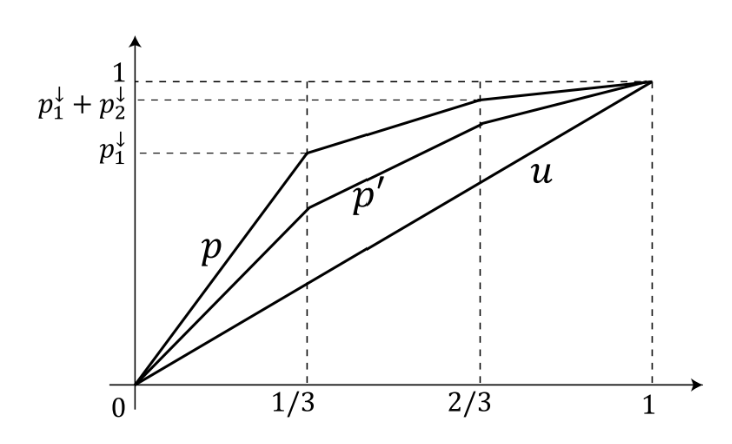
\includegraphics[width=100mm]{image1.png}
    \end{center}
    \caption{Majorizationの図示}
    \label{fig:one}
\end{figure}
図でいうところの、下に来ている曲線が、よりばらつきが小さい確率分布であり、とくに一様分布のときは直線になることがわかる。すなわち、
\begin{equation}
    u \prec p \quad \forall p \in \mathcal{P}_d
\end{equation}
である。\\
注意すべきこととして、この$\prec$は全順序ではない。すなわち、ある確率分布の組$p,p'$に対して、$p \prec p'$か$p' \prec p$のどちらも成り立たない場合がある。このとき、ローレンツ曲線は交わる。\\

\begin{itembox}[l]{\textbf{Thm:Majorizationの特徴づけ}}
    $p,p' \in \mathcal{P}_d$に対して、以下は同値である。
    \begin{enumerate}
        \item $p' \prec p$
        \item $\forall t\in \mathbb{R} \quad \sum_{i=1}^{d}|p_i'-t| \leq \sum_{i=1}^{d}|p_i-t|$
        \item 任意の下に凸な関数$f$に対して、
        \begin{equation}
            \sum_{i=1}^{d}f(p_i') \leq \sum_{i=1}^{d}f(p_i)
        \end{equation}
        \item $p' = Tp$となる二重確率遷移行列$T$が存在する。
    \end{enumerate}
\end{itembox}
\textbf{Prf}\\
この証明は後で行う。\\

\textbf{3についての補足}
%後で書く。\\

また、一様分布は、二重確率遷移行列のもとで不変である。熱力学の文脈では、uは高温極限をとった時のGibbs分布に対応している。このとき、二重確率遷移行列は、そのようなGibbs分布を保つものである。\\

\begin{itembox}[l]{\textbf{Thm:Birkhoffの定理}}
    以下の二つは同値である。
    \begin{enumerate}
        \item $T$は二重確率遷移行列である。
        \item $T$は、置換行列の凸結合で表現できる。すなわち、
        \begin{equation}
            T = \sum_{k} r_k P_k
        \end{equation}
        である。ただし、$r_k \geq 0$であり、$\sum_k r_k = 1$である。また、$P_k$は、置換行列である。
    \end{enumerate}
\end{itembox}
\textbf{Prf}\\
教科書で証明されていないので一旦飛ばす。\\

\begin{itembox}[l]{\textbf{Prop:二重確率遷移行列の性質}}
    \begin{equation}
        「Tが二重確率遷移行列である」 \Leftrightarrow Tp \prec p \quad \forall p \in \mathbb{R}^d
    \end{equation}
\end{itembox}
\textbf{Prf}\\
%後で書く。\\

\begin{itembox}[l]{\textbf{Def:Schur凸性}}
    $F: \mathbb{R}^d \to \mathbb{R}$がSchur凸であるとは、
    \begin{equation}
        \forall p,p' \in \mathcal{P}_d \quad p' \prec p \Rightarrow F(p') \leq F(p)
    \end{equation}
    が成り立つことである。言い換えると、Schur凸な関数は、majorizationに関して単調である。
\end{itembox}

\begin{itembox}[l]{\textbf{Prop:}}
    $F: \mathbb{R}^d \to \mathbb{R}$がSchur凸かつ微分可能なことと、Fが転置に対して不変なこと、すなわち、
    \begin{equation}
        F(p) = F(Pp) \quad \forall p ,P
    \end{equation}
    が成り立つことは同値であり、また、
    \begin{equation}
        \forall p \in \mathcal{P}_d \quad (p_ip_j)\left(\pdv{F}{p_i}-\pdv{F}{p_j}\right)\geq 0
    \end{equation}
    も同値である。
\end{itembox}
\textbf{Prf}\\
%後で書く。\\

\subsection{d-MajorizationとThermo-Majorization}
先ほどまでは、一つの分布についての遷移について考えていたが、次は、二つの分布の組の遷移を考える。\\
このとき、$p^*=(p_1^*,...,p_d^*)^{\top},q^*=(q_1^*,...,q_d^*)^{\top}$を、$p=(p_1,...,p_d)^{\top},q=(q_1,...,q_d)^{\top}$を
$\frac{p_1^*}{q_1^*} \geq \frac{p_2^*}{q_2^*} \geq ... \geq \frac{p_d^*}{q_d^*}$が成り立つように並べ替えたものとして定義する。この新しく定義した$p^*,q^*$に対して
横軸を$\sum_{i=1}^{k}q_i^*$、縦軸を$\sum_{i=1}^{k}p_i^*$としたローレンツ曲線を考える。図は以下のようになる。\\
\begin{figure}[H]
    \begin{center}
    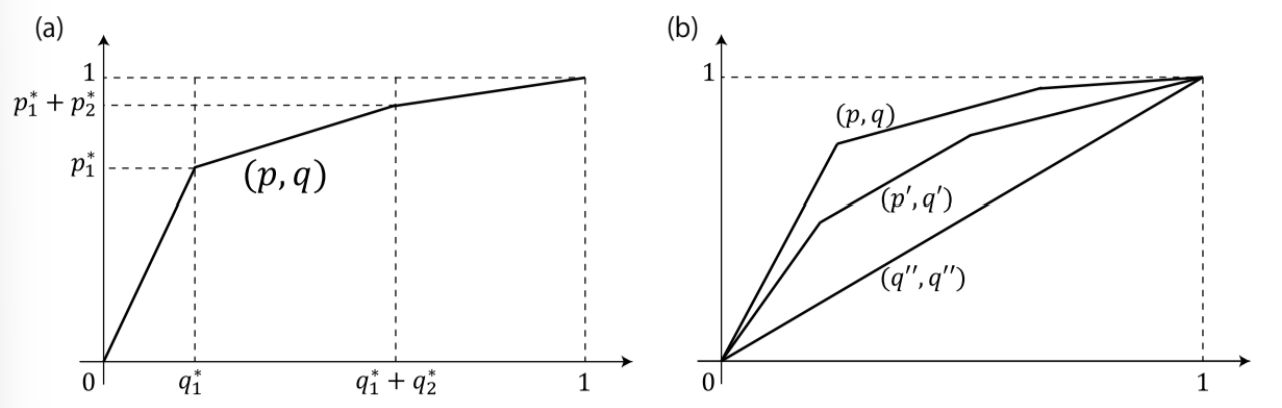
\includegraphics[width=100mm]{image2.png}
    \end{center}
    \caption{d-Majorizationの図示}
    \label{fig:two}
\end{figure}

\begin{itembox}[l]{\textbf{Def:d-Majorization}}
    $p,q,p',q' \in \mathcal{P}_d$に対して、
    \begin{equation}
        (p',q') \prec (p,q) \Leftrightarrow 「(p,q) \text{のローレンツ曲線が}(p',q') \text{のローレンツ曲線の上に来る」}
    \end{equation}a
    が成り立つとき、$(p,q)$は$(p',q')$をd-majorizeするという。
\end{itembox}
d-majorizationは、以下のような言いかえが可能である。\\
\begin{itembox}[l]{\textbf{Thm:Blackwellの定理}}
    $p,q,p',q' \in \mathcal{P}_d$かつ$q,q'$がフルランクであるとき、以下は同値である。
    \begin{enumerate}
        \item $(p',q') \prec (p,q)$
        \item 
        \begin{equation}
            \forall t \in \mathbb{R} \quad \sum_{i=1}^{d}|p_i'-tq_i'| \leq \sum_{i=1}^{d}|p_i-tq_i|
        \end{equation}
        \item 任意の下に凸な関数$f$に対して、
        \begin{equation}
            \sum_{i=1}^{d} q_i'f(\frac{p_i'}{q_i'}) \leq \sum_{i=1}^{d} q_i f(\frac{p_i}{q_i})
        \end{equation}
        \item ある二重確率遷移行列$T$が存在して、
        \begin{equation}
            p' = Tp \quad q' = Tq
        \end{equation}
        が成り立つ。
    \end{enumerate}
\end{itembox}
\textbf{Prf}\\
後で証明を行う。\\



\begin{itembox}[l]{\textbf{Def:Thermo-Majorization}}
    $p,q,p' \in \mathcal{P}_d$に対して、pがqについてp'をthermo-majorizeするとは、
    \begin{equation}
        (p',q) \prec (p,q)
    \end{equation}
    が成り立つことである。
\end{itembox}
$(q,q)$のローレンツ曲線は、直線であるため、$q$は任意の$p$についてthermo-majorizeされる。すなわち、
\begin{equation}
    \forall p \quad (q,q) \prec (p,q)
\end{equation}
である。したがって、thermo-majorizationは、確率分布$p$が$q$にどれだけ近いかを表す。\\
とくに、熱力学の文脈では$q$はあるハミルトニアン$H$のGibbs分布であり、$q=p^G$とかける。\footnote{任意のフルランクな$q$はあるハミルトニアンのGibbs分布であるらしい。}
このとき、$q=Tq$であるとは、$T$は、Gibbs分布を変えない遷移行列であるということである。このような遷移行列を、Gibbs-preserving mapという。\\
リソース理論の枠組みでは、GPMは、free operationとして扱われ、Gibbs分布は、free stateとして扱われる。\\

\begin{itembox}[l]{\textbf{Thm:遷移可能条件}}
    $p,q,p',q' \in \mathcal{P}_d$とし、$q,q'$がフルランクであるとする。このとき、以下の二つが成り立つ。
    \begin{enumerate}
        \item
        \begin{equation}
            (p',q') \prec (p,q) \Leftrightarrow S_0(p||q) \geq S_0(p'||q') \quad S_{\infty}(p||q) \leq S_{\infty}(p'||q')
        \end{equation}
        \item
        \begin{equation}
            S_{\infty}(p'||q') \leq S_{0}(p||q) \Leftrightarrow (p',q') \prec (p,q)
        \end{equation}
    \end{enumerate}

\end{itembox}
\textbf{Prf}\\
以下の図より明らかである。%TODO後で見る。\\
\begin{figure}[H]
    \begin{center}
    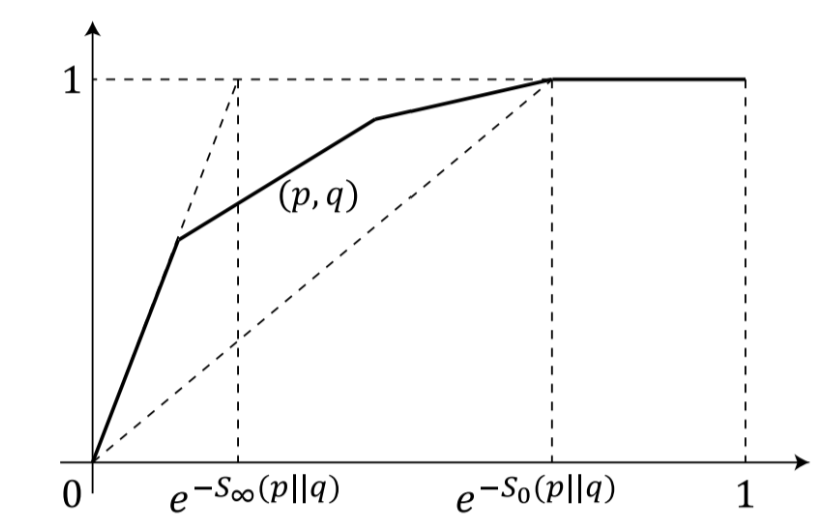
\includegraphics[width=100mm]{image3.png}
    \end{center}
    \caption{遷移可能条件の図示}
    \label{fig:three}
\end{figure}
上の定理から明らかなように、Rényi divergence の観点からは,状態遷移と d-majorization に関する必要条件と十分条件は一致しない。\\

%\subsection{Catalytic Majorization}
%状態変化の際に、触媒と呼ばれる量が関与する場合を考える。このとき、状態変化の前後で触媒の状態が変化しないことに注意したい。\\

\subsection{連続変数の場合}
Majorizationおよびd-majorizationの連続変数の場合を考える。\\
簡単のため、$x\in[0,1]$とする。
%必要であれば地の文を追加する。

\begin{itembox}[l]{\textbf{Def:連続変数におけるMajorization}}
    $p,p' \in L^1([0,1])$に対して、$p$が$p'$をmajorizeすることを、$p' \prec p$と書き、
    \begin{equation}
        \forall y \in [0,1] \quad \int_{0}^{y}{p'}(x)^{\downarrow}dx \leq \int_{0}^{y}p(x)^{\downarrow}dx
    \end{equation}
    が成り立つとき、$p$が$p'$をmajorizeするという。ただし、
    \begin{align}
        p^{\downarrow}(x) =\sup \{y: m_p(y) >x\}\\
        m_p(y) = \mu[x:p(x)>y]\\
        \mu : \text{Lebesgue measure}
    \end{align}
    である。\footnote[1]{ルベーグ積分が分からないせいで全然納得できない。}
\end{itembox}

\begin{itembox}[l]{\textbf{Def:二重確率遷移写像}}
    $T:L^1([0,1]) \to L^1([0,1])$が二重確率遷移写像であるとは、
    \begin{equation}
        \forall p \in L^1([0,1]) \quad Tp \prec p
    \end{equation}
    が成り立つことである。
\end{itembox}
%TODOルベーグ積分がわからないので一旦この節は飛ばす。

\newpage
\section{古典熱力学への適応}
古典熱力学との対応を見ていく。
\subsection{第二法則とKLダイバージェンス}
熱力学第二法則が、KLダイバージェンスの単調性に由来することを確認する、\\
$E_i$を、系の$i$番目の状態のエネルギーとし、Gibbs状態$p^G \in \mathcal{P}_d$を、$p^G_i = \frac{e^{-\beta E_i}}{Z}$で定義する。ただし、$Z$は正規化定数である。
また、平衡状態での自由エネルギーは、$F = -\beta^{-1}\log Z$である。\\
また、GPMは、
\begin{equation}
    p^G = Tp^G
\end{equation}
であった。\\
\begin{itembox}[l]{\textbf{Prop:詳細つり合い条件とGPM}}
    系が詳細つり合い条件
    \begin{equation}
        T_{ji} e^{-\beta E_i} = T_{ij} e^{-\beta E_j}
    \end{equation}
    を満たすならば、$T$はGPMである。
\end{itembox}
\textbf{Prf}\\
\begin{align}
    \sum_j T_{ij}p_j &= \sum_j T_{ji}p_i\\
    &= p_i \quad (\because \sum_j T_{ji} = 1)
\end{align}
からわかる。\hfill \qedsymbol\\

以下、$\beta \geq 0$を逆温度とする。KLダイバージェンスの単調性を用いると、
\begin{align}
    S_1(p||p^G) \geq S_1(Tp||p^G)\\
\end{align}
となることがわかる。KLダイバージェンスの定義より、
\begin{align}
    S_1(p||p^G) &= \sum_{i=1}^{d}p_i\log\left(\frac{p_i}{p_i^G}\right)\\
    &= \sum_{i=1}^{d}p_i\log(p_i) + \beta \sum_{i=1}^{d}p_i E_i\\
    &= -S(p) + \beta \sum_{i=1}^{d}p_i E_i
\end{align}
同様にして、
\begin{align}
    S_1(Tp||p^G) &= -S(Tp) + \beta \sum_{i=1}^{d}(Tp)_i E_i\\
\end{align}
である。したがって、
\begin{equation}
    S(Tp) - S(p) \geq \beta (\sum_{i=1}^{d}E_i(Tp)_i - \sum_{i=1}^{d}E_ip_i)
\end{equation}
である。右辺を観察してみると、遷移前後のエネルギーの期待値の差が現れていることがわかる。ここで、
\begin{equation}
    Q = \sum_{i=1}^{d}E_i(Tp_i - \sum_{i=1}^{d}E_ip_i)
\end{equation}
と定義すると、
\begin{equation}
    \Delta S =S(Tp) - S(p) \geq \beta Q
\end{equation}
と書くことができる。これは、クラウジウス不等式と呼ばれ、熱力学第二法則を表す。ただし、注意したいこととしては、左辺はシャノンエントロピーという、情報理論の文脈でのエントロピーである。\\
以上の議論を踏まえると、$T$という、Gibbs分布を保つ遷移がおこるとき、分布を保つために熱浴との相互作用が起こり、エントロピーが増大することがわかる。\\
\textbf{Rem}\\
上の熱について、$Q_{ji} =E_j-E_i$を、状態jからiへの遷移の際の熱の変化量とすると、
\begin{equation}
    Q = \sum_{i,j}T_{ji}p_iQ_{ji}
\end{equation}
と書くことができる。%TODOここの意味を後でとる。

確率熱力学の文脈では、
\begin{equation}
    \Sigma = S_1(p||p^G)-S_1(Tp||p^G)=\Delta S - \beta Q \geq 0
\end{equation}
をエントロピー生成と呼ぶ。とくに、$\Delta S-\beta Q$は、熱浴のエントロピー増加ととらえられる。\\
%地の文を書くかもしれない。

つぎに、仕事と自由エネルギーについての第二法則を見ていく。いま、系のハミルトニアンは時間依存するとし、系への仕事はハミルトニアンの時間変化により実現されるとする。
ここで、ハミルトニアンは、仕事浴によって変化するのではなく、外部操作によって駆動すると考える。\\
まず、クエンチによって駆動される系を考える。いま、$E =\sum_{i}E_i p_i$, $E' = \sum_{i}E'_i p_i$がクエンチ前後での系のエネルギーの期待値あるとする。また、クエンチによってなされる仕事の平均は、
\begin{equation}
    W = E'-E
\end{equation}
と書かれる。\\
\textbf{Rem}\\
このセットアップでは、仕事は揺らぐ量であることに注意したい。すなわち、確率的な仕事を$w_i = E'_i - E_i$として、
\begin{equation}
    W = \sum_{i}w_i p_i
\end{equation}
である。\\

次に、より一般的な熱力学過程を考える。全体の過程が、複数のクエンチおよび緩和過程によって構成されると考える。クエンチとクエンチの間では、ハミルトニアンは一定であるとする。\\
また、各緩和過程は確率的に独立であるとし、そのときのハミルトニアンに対応するGPMによって記述されると仮定する。
以上の過程を図示すると以下のようになる。
\begin{figure}[H]
    \begin{center}
    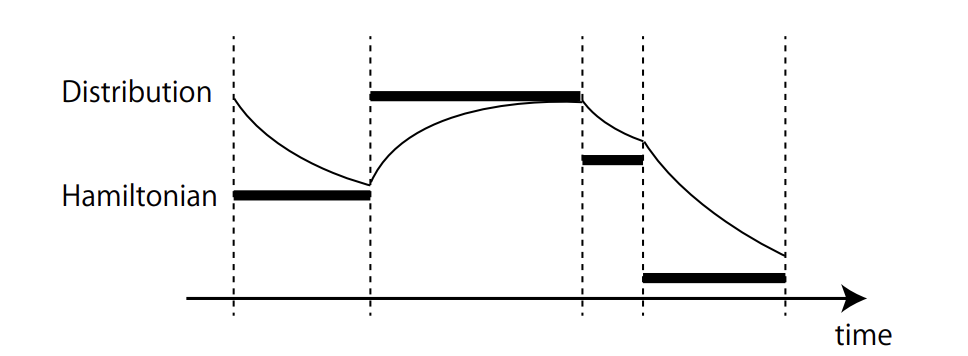
\includegraphics[width=100mm]{image4.png}
    \end{center}
    \caption{熱力学過程の図示}
    \label{fig:four}
\end{figure}
全体の過程についての始状態と終状態を$p,p'$とし、ハミルトニアンを$H,H'$とする。また、Gibbs状態を$p^G,p'^G$として、ヘルムホルツ自由エネルギーを$F,F'$とする。\footnote{この自由エネルギーは、熱平衡状態にある時の自由エネルギーであることに注意されたい。}\\
上の過程における、平均の仕事と熱について考える。$\Delta E = E'-E$、$E =\sum_{i}E_i p_i$, $E' = \sum_{i}E'_i p_i$とすると熱力学第一法則が成り立つ。すなわち、
\begin{equation}
    \Delta E = W + Q
\end{equation}
が成立する。このとき、クエンチは、一瞬で行われるので、その間に確率分布は変化せず、また、熱の交換も起こらないとみなせる。したがって、この過程において、熱力学第一法則に影響はない。\\
この第一法則を用いると、第二法則は、
\begin{equation}
    W \geq \Delta E - \beta^{-1}\Delta S_1
\end{equation}
と書くことができる。ここで、非平衡状態における自由エネルギーを以下のように定義する。
\begin{equation}
    F_1(p;H) = \Delta E_i - \beta^{-1}\Delta S_1(p) = \beta^{-1}S_1(p||p^G) + F
\end{equation}
このとき、
\begin{equation}
    F_1(p;H) = F \Leftarrow p = p^G
\end{equation}
である。この自由エネルギーの表式を用いることにより、
\begin{equation}
    W \geq F_1(p';H') - F_1(p;H)
\end{equation}
と書くことができる。この不等式は、仕事の揺らぎを許すときの仕事の下限を与える。\\
%準静的過程のときの話とかをここに追加する。

\subsection{非平衡状態への遷移の要する仕事}
非平衡状態へ遷移する際に必要な仕事を、Thermo-Majorizationを用いて考える。\\
$p^G$を、系のGibbs分布とし、$p_{i}^G = \frac{e^{-\beta E_i}}{Z}$で定義する。また、$p$を、系の任意の状態とする。また、今、仕事浴が、二つのエネルギー準位$0,w$を持つとする。
仕事浴のGibbs分布を$r^G$とし、$r^G = (\frac{1}{1+e^{-\beta w}},\frac{e^{-\beta w}}{1+e^{-\beta w}})^{\top}$とし、また、仕事浴の任意の状態を$r=(r_0,r_w)^{\top} \quad r_0+r_w=1$とする。\\
また、はじめと最後の仕事浴のエネルギーが$0$か$w$で与えられているとして、エネルギーの変化はすべて$w$か$-w$であるとする。

以下、非平衡状態を作るための最小仕事を求める。ここで、系のハミルトニアンが初めと終わりで等しいことを仮定する。\\
始状態の系の確率分布は$p^G$であり、仕事浴の確率分布は、$r^{up} = (0,1)$であるとする。このとき、SW系(着目系と仕事浴の合成系)の初期状態は、$p^G \otimes r^{up}$である。\\
また、終状態について、終状態の系の状態を$p$、仕事浴の状態を$r^{down} = (1,0)$とする。このとき、SW系の終状態は、$p \otimes r^{down}$である。\\
このとき、それぞれのテンソル積を書き下すと以下のようになる。
\begin{align}
    p^G \otimes r^{up} &= (0,p_1^G,0,p_2^G,\cdots,0,p_n ^G)\\
    p \otimes r^{down} &= (p_1,0,p_2,0,\cdots,p_n,0)
\end{align}
また、ローレンツ曲線を書くために、$p^G \otimes r^G$を書き下すと、
\begin{equation}
    p^G \otimes r^G = (p_1^G r^{G,down},p_1^G r^{G,up},p_2^G r^{G,down},p_2^G r^{G,up},\cdots,p_n^G r^{G,down},p_n^G r^{G,up})
\end{equation}
である。ここで、$r^{G,up} = \frac{1}{1+e^{-\beta w}}$、$r^{G,down} = \frac{e^{-\beta w}}{1+e^{-\beta w}}$である。\\
以上の準備の下、ローレンツ曲線を描くことを考える。まず、初期状態についてのローレンツ曲線は、要素が0でないところから大きい順に足していけばよいことがわかる。また、終状態については、折れ線となる。これらを図示すると以下のようになる。
\begin{figure}[H]
    \begin{center}
    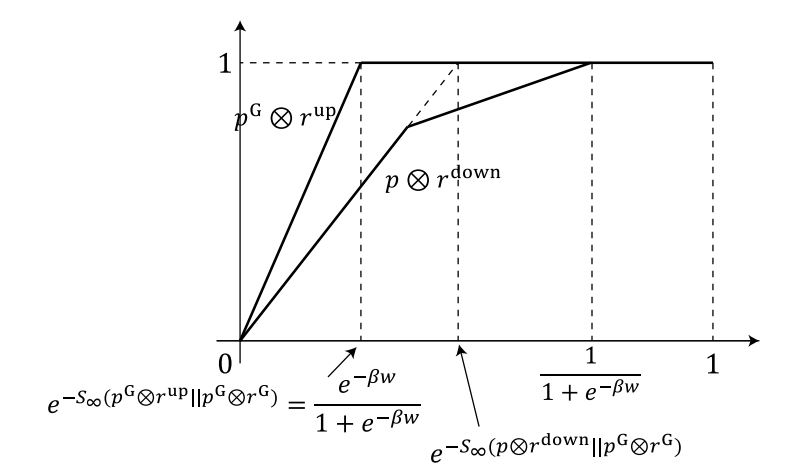
\includegraphics[width=100mm]{image5.png}
    \end{center}
    \caption{非平衡状態への遷移の図示}
    \label{fig:five}
\end{figure}
したがって、非平衡状態への遷移が可能な必要十分条件は、
\begin{equation}
    \frac{e^{-\beta w}}{1+e^{-\beta w}} \leq e^{-S_{\infty} (p\times r^{down}||p^G \times r^G)}
\end{equation}
である。ここで、
\begin{align}
    S_{\infty} (p\otimes r^{down}||p^G \otimes r^G) &= \ln (\underset{i}{\max}\frac{p_i\otimes r^{down}}{p_i^G \otimes r^{G,down}})\\
    &= \ln (\underset{i}{\max}\frac{p_i}{p_i^G})-\ln(r^{G,down})\\
    &= S_{\infty}(p||p^G) - \ln(r^{G,down})
\end{align}
であることを用いると、
\begin{equation}
    \frac{e^{-\beta w}}{1+e^{-\beta w}} \leq \frac{1}{1+e^{-\beta w}}e^{-S_{\infty}(p||p^G)}
\end{equation}
となる。整理して、
\begin{equation}
    w \geq \beta^{-1}S_{\infty}(p||p^G)
\end{equation}
となる。これが、平衡系から非平衡系への遷移に必要な最小仕事である。\\

\subsection{熱平衡状態への緩和で取り出せる仕事}
上と同様のことを考える。疲れたので図と結果だけを書く。\\
\begin{figure}[H]
    \begin{center}
    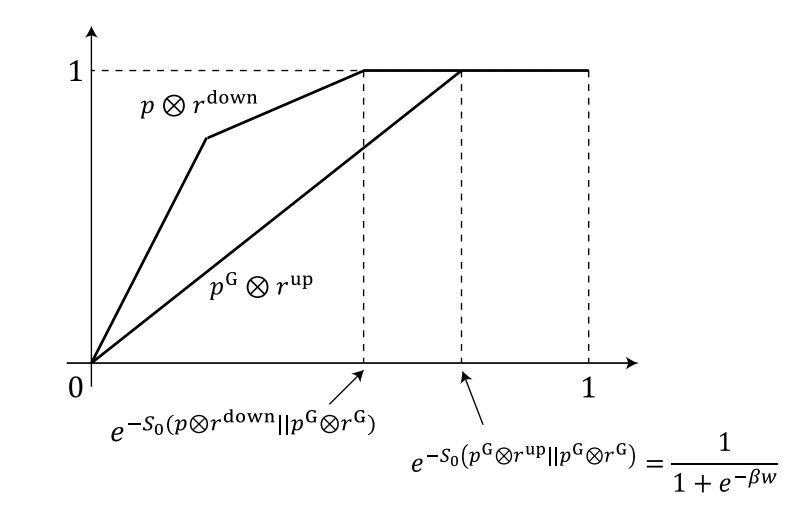
\includegraphics[width=100mm]{image6.png}
    \end{center}
    \caption{熱平衡状態への緩和の図示}
    \label{fig:six}
\end{figure}
\begin{equation}
    -w \leq \beta^{-1}S_{0}(p||p^G)
\end{equation}
である。これが、非平衡系から平衡系への遷移において取り出せる最大仕事である。\\

この等号が成り立つようなプロトコルが本文にあるが、クエンチしている時点でセットアップがよくわからん。外部系から操作しているように見えてしまう。\\
ただまあ、仕事の揺らぎがある系(i.e.確率熱力学に従う系)は、その揺らぎを許さない形よりも効率が悪い気がする(カルノーサイクルの隔離る熱力学での話を思い出す)ので、原理的限界としてとりあえずリソース理論を用いていて、
たまたまそれを達成する操作を確率熱力学の文脈からも出せるという話である気もしてくる。

\subsection{平衡状態間の遷移における仕事}
最後に、Gibbs分布間の状態の遷移を考える。このとき、clockと呼ばれる機構により、ハミルトニアンを時間変化させる。\\
系のハミルトニアンについて、clockが0のときは、$E_i$、clockが1のときは、$E'_i$であるとする。また、はじめと最後の確率分布を$p,p'$とする。ただし、
\begin{align}
    p_i &= \frac{e^{-\beta E_i}}{Z}\\
    p'_i &= \frac{e^{-\beta E'_i}}{Z'}
\end{align}
である。\\
また、それに対応する自由エネルギーは、
\begin{align}
    F &= -\beta^{-1}\log Z\\
    F' &= -\beta^{-1}\log Z'
\end{align}
である。\\
以下、簡単のために、clockは$0$か$1$の値のみを取るとする。初め、$C(clock)=(1,0)$であり、終わりには$C(clock)=(0,1)$であるとする。\\
このとき、保存するGibbs分布は、
\begin{align}
    p_{SC}^G = \frac{Z}{Z+Z'}p \otimes c + \frac{Z'}{Z+Z'}p' \otimes c'
\end{align}
である。\\
$\because$\\
%TODO後で書く。よくわかってない。

以上の準備の下、Majorizationを用いる。$p_{SC}^G \otimes r^{up}$と$p_{SC}^G \otimes r^{down}$について、Majorizationを考える。このとき、どちらもGibbs分布であるからどちらも直線となる:

\begin{figure}[H]
    \begin{center}
    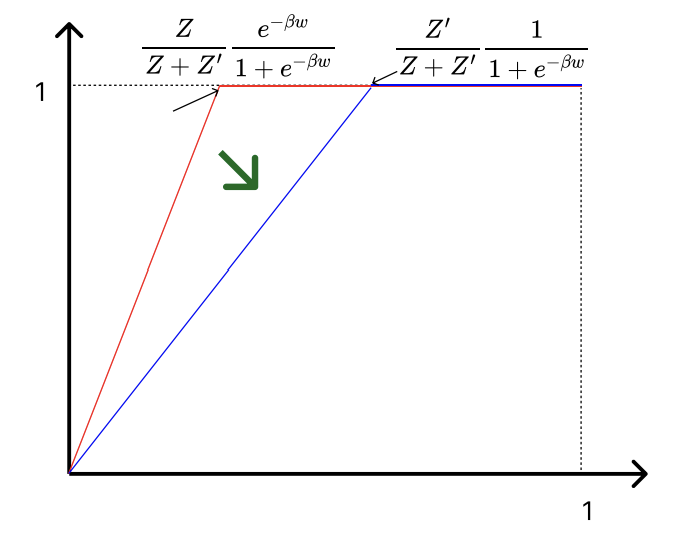
\includegraphics[width=70mm]{image7.png}
    \end{center}
    \caption{平衡状態間の遷移の図示}
    \label{fig:seven}
\end{figure}
このとき$p$が$p'$をthermo-majorizeする条件は、
\begin{equation}
    \frac{Z}{Z+Z'}\frac{e^{-\beta w}}{1+e^{-\beta w}} \leq \frac{Z'}{Z+Z'}\frac{1}{1+e^{-\beta w}}
\end{equation}
である。これを整理することで、
\begin{equation}
    w \geq \Delta F
\end{equation}
となる。これが、平衡状態間の遷移における最小仕事であり、たしかに熱力学第二法則が再現されることがわかる。\\

\newpage
\section{量子エントロピー及びダイバージェンス}
\subsection{量子状態及び系}
量子状態とかの話を確認する。\\

\begin{itembox}[l]{\textbf{Def:完全正値写像}}
    線形写像 $\mathcal{E} : \mathcal{L}(\mathcal{H}) \rightarrow \mathcal{L}(\mathcal{H}')$ について:

\begin{itemize}
  \item $\mathcal{E}$は正値であるとは、任意の演算子が正値演算子に写像されることを意味する。すなわち、$\hat{X} \geq 0$ ならば $\mathcal{E}(\hat{X}) \geq 0$である。
  \item $\mathcal{E}$がn-positiveであるとは、$\mathcal{E} \otimes \mathcal{I}_n$が正値であることを意味する。ここで $\mathcal{I}_n$ は $\mathcal{L}(\mathbb{C}^n)$ 上の恒等超演算子である。
  \item $\mathcal{E}$がCPであるとは、すべての $n \in \mathbb{N}$ に対してn-positiveであることを意味する。
\end{itemize}

\end{itembox}

\begin{itembox}[l]{\textbf{Def:トレース保存性}}
    線形写像 $\mathcal{E} : \mathcal{L}(\mathcal{H}) \rightarrow \mathcal{L}(\mathcal{H}')$ について、$\mathcal{E}$がトレース保存であるとは、
    \begin{equation}
        \text{Tr}[\mathcal{E}(\hat{X})] = \text{Tr}[\hat{X}]
    \end{equation}
    が成り立つことを意味する。
\end{itembox}
このとき、確率保存を満たすような任意の状態の写像はCPTP写像である。\\

\begin{itembox}[l]{\textbf{Prop:Kraus表現}}
    超演算子 $\mathcal{E} : \mathcal{L}(\mathcal{H}) \rightarrow \mathcal{L}(\mathcal{H}')$ がCPであるための必要十分条件は、
    \begin{equation}
        \mathcal{E}(\hat{\rho}) = \sum_{k} \hat{M}_k \hat{\rho} \hat{M}_k^{\dagger}
    \end{equation}
    と表現できることである。ここで、$\hat{M}_k$はKraus演算子であり、
    \begin{equation}
        \sum_{k} \hat{M}_k^{\dagger} \hat{M}_k = \hat{I}
    \end{equation}
    が成り立つ。これにより、トレース保存性が保証される。

\end{itembox}

\begin{itembox}[l]{\textbf{Def:ユニタル写像}}
    $\mathcal H$をヒルベルト空間とし、$\mathcal{E} : \mathcal{L}(\mathcal{H}) \rightarrow \mathcal{L}(\mathcal{H})$ がユニタルであるとは、
    \begin{equation}
        \mathcal{E}(I) = I
    \end{equation}
    を満たすことを意味する。ここで、$I$は恒等演算子である。
\end{itembox}

\begin{itembox}[l]{\textbf{Def:Hilbert-Schmidt内積}}
    ヒルベルト空間$\mathcal{H}$上の演算子$\hat{A},\hat{B}$に対して、Hilbert-Schmidt内積を以下のように定義する:
    \begin{equation}
        \langle \hat{Y},\hat{X} \rangle_{HS} = \text{Tr}[\hat{Y}^{\dagger}\hat{X}]
    \end{equation}

\end{itembox}
また、これを用いて、$\mathcal{E}$のエルミート共役を以下のように定義する。
\begin{itembox}[l]{\textbf{Def:$\mathcal{E}$のエルミート共役}}
    $\mathcal{E} : \mathcal{L}(\mathcal{H}) \rightarrow \mathcal{L}(\mathcal{H})$ に対して、$\mathcal{E}$のエルミート共役$\mathcal{E}^{\dagger}$は、
    \begin{equation}
        \langle Y,\mathcal{E}(X) \rangle_{HS} = \langle \mathcal{E}^{\dagger}(Y),X \rangle_{HS}
    \end{equation}
    を満たすような線形写像である。

\end{itembox}

\begin{itembox}[l]{\textbf{Prop:}}
    $\mathcal E$がTP写像であることと、$\mathcal E^{\dagger}$がユニタル写像であることは同値である。
\end{itembox}
\textbf{Prf}\\
\begin{align}
    \Trace[\mathcal E(\hat X)] &= \ev{\hat{I},\mathcal E(\hat X)}_{HS}\\
    &= \ev{\mathcal E^{\dagger}(\hat I),\hat X}_{HS}\\
    &= \Trace[\mathcal E^{\dagger}(\hat I)\hat X]
\end{align}
であるから、示された。\hfill \qedsymbol\\

\begin{itembox}[l]{\textbf{Prop:}}
    $\mathcal E$がCP写像であることと、$\mathcal E^{\dagger}$がCP写像であることは同値である。

\end{itembox}
\textbf{Prf}\\
%TODO後で書く。

最後に、演算子のノルムについて言及する。$\hat{X}$を$\mathcal{H}$上で作用する任意の演算子とする。まず、トレースノルムは次のように定義する。
\begin{equation}
\|\hat{X}\|_1 := \operatorname{tr}[|\hat{X}|],
\end{equation}
ここで、$|\hat{X}| := \sqrt{\hat{X}^\dagger \hat{X}}$である。これは数学的意味でのノルムであり、三角不等式$\|\hat{X} + \hat{X}'\|_1 \leq \|\hat{X}\|_1 + \|\hat{X}'\|_1$を満たし、$\|\hat{X}\|_1 = 0$が$\hat{X} = 0$のときかつそのときに限り成り立つ。トレース距離は次のように定義する。
\begin{equation}
D(\hat{\rho}, \hat{\sigma}) := \frac{1}{2} \|\hat{\rho} - \hat{\sigma}\|_1,
\end{equation}
これは量子状態$\hat{\rho}$と$\hat{\sigma}$の間の距離を測定するために一般的に使用され、CPTP写像$\mathcal{E}$の下での単調性を満たす([4]の定理9.2)。
\begin{equation}
D(\hat{\rho}, \hat{\sigma}) \geq D(\mathcal{E}(\hat{\rho}), \mathcal{E}(\hat{\sigma})).
\end{equation}

もう一つの重要なノルムは演算子ノルムで、次のように定義する。
\begin{equation}
\|\hat{X}\|_\infty := \max_{\|\phi\|=1} \sqrt{\langle \phi | \hat{X}^\dagger \hat{X} | \phi \rangle},
\end{equation}
これは$\hat{X}$の最大の特異値に他ならない。

\newpage
\section{von Neumannエントロピー/量子KLダイバージェンス}

\begin{itembox}[l]{\textbf{Def:von Neumannエントロピー}}
        量子状態$\hat{\rho}$のvon Neumannエントロピーは、
        \begin{equation}
            S(\hat{\rho}) = -\Trace[\hat{\rho}\log \hat{\rho}]
        \end{equation}
        で定義される。

\end{itembox}

このとき、密度行列はエルミートなので、対角化可能である。すなわち、ヒルベルト空間$\mathcal{H}$の基底をうまく選ぶことで、
\begin{equation}
    \hat{\rho} = \sum_{i} p_i \ket{i}\bra{i}
\end{equation}
と書くことができる。このとき、von Neumannエントロピーは、
\begin{equation}
    S(\hat{\rho}) = -\sum_{i} p_i \log p_i
\end{equation}
と書くことができ、これはシャノンエントロピーと一致する。\\
また、トレースの巡回性から、
\begin{equation}
    S(\hat{\rho}) = S(U\hat{\rho}U^{\dagger})
\end{equation}
が成り立つ。\\
これと、シャノンエントロピーの性質から、
\begin{equation}
    0 \leq S(\hat{\rho}) \leq \log d
\end{equation}
が成り立つ。ここで、$d$はヒルベルト空間の次元である。\\

\begin{itembox}[l]{\textbf{Def:量子KLダイバージェンス}}
    量子状態$\hat{\rho},\hat{\sigma}$のKLダイバージェンスは、
    \begin{equation}
        S_1(\hat{\rho}||\hat{\sigma}) = \Trace[\hat{\rho}(\log \hat{\rho} - \hat{\rho}\log \hat{\sigma})]
    \end{equation}
    で定義される。
\end{itembox}
このとき、簡単な計算により、
\begin{equation}
    S_1(\hat{\rho}) =\ln d - S(\hat{\rho}||{\frac{\hat{{I}}}{d}})
\end{equation}
が成り立つ。\\
また、もし$\hat{\rho},\hat{\sigma}$が同じ基底を用いて展開できるとき、量子KLダイバージェンスは、古典的なKLダイバージェンスと一致する。\\
また、トレースの巡回性から、
\begin{equation}
    S_1(\hat{\rho}||\hat{\sigma}) = S_1(U\hat{\rho}U^{\dagger}||U\hat{\sigma}U^{\dagger})
\end{equation}
が成り立つ。\\
また、量子KLダイバージェンスは、非負である。すなわち、
\begin{equation}
    S_1(\hat{\rho}||\hat{\sigma}) \geq 0
\end{equation}
が成り立つ。\\
%TODO証明を後で書く

\begin{itembox}[l]{\textbf{Thm:単調性}}
    量子状態$\hat{\rho},\hat{\sigma}$に対して、
    \begin{equation}
        S_1(\hat{\rho}||\hat{\sigma}) \geq 0
    \end{equation}
    が成り立つ。また、
    \begin{equation}
        S_1(\hat{\rho}||\hat{\sigma}) \geq S_1(\mathcal{E}(\hat{\rho})||\mathcal{E}(\hat{\sigma}))
    \end{equation}
    が成り立つ。ここで、$\mathcal{E}$はCPTP写像である。

\end{itembox}
\textbf{Prf}\\
略。\hfill \qedsymbol\\

\begin{itembox}[l]{\textbf{Prop:}}
    $\mathcal{E}$がユニタル写像であるならば、
    \begin{equation}
        S_1(\hat{\rho}) \leq S_1(\mathcal{E}(\hat{\rho}))
    \end{equation}
    が成り立つ。
\end{itembox}
\textbf{Prf}\\
von Neumannエントロピーと量子ダイバージェンスの関係式及び、量子ダイバージェンスの単調性を用いることで示される。\hfill \qedsymbol\\

\begin{itembox}[l]{\textbf{Prop:von Neumannエントロピーの劣加法性}}
    量子状態$\hat{\rho}_A,\hat{\rho}_B$に対して、
    \begin{equation}
        S_1(\hat{\rho}_{AB}) \leq S_1(\hat{\rho}_A) + S_1(\hat{\rho}_B)
    \end{equation}
    が成り立つ。
\end{itembox}
\textbf{Prf}\\
量子KLダイバージェンスの定義および非負性を用いることで、
\begin{equation}
S_1(\hat{\rho}_{A}) + S_1(\hat{\rho}_{B}) - S_1(\hat{\rho}_{AB}) = S_1(\hat{\rho}_{AB}||\hat{\rho}_{A} \otimes \hat{\rho}_{B}) \geq 0
\end{equation}
が示される。\hfill \qedsymbol\\
また、等号成立は、$\hat{\rho}_{AB} = \hat{\rho}_{A} \otimes \hat{\rho}_{B}$のときに成り立つ。\\

証明の第一式は、
\begin{align}
    I_1(\hat{\rho}_{AB}) := S_1(\hat{\rho}_{A}) + S_1(\hat{\rho}_{B}) - S_1(\hat{\rho}_{AB})\\
\end{align}
とかき、相互情報量の性質という。\\

\begin{itembox}[l]{\textbf{prop:強劣加法性}}
    部分系$A,B,C$に対して、
    \begin{equation}
        S_1(\hat{\rho}_{ABC}) + S_1(\hat{\rho}_B) \leq S_1(\hat{\rho}_{AB}) + S_1(\hat{\rho}_{BC})
    \end{equation}
    が成り立つ。
\end{itembox}
\textbf{Prf}\\
量子KLダイバージェンスの単調性を用いる。\\
\begin{align}
    S_1(\hat{\rho}_{AB}) + S_1(\hat{\rho}_{BC}) - S_1(\hat{\rho}_{ABC}) - S_1(\hat{\rho}_B) 
    &=[S_1(\hat{\rho}_{BC}) - S_1(\hat{\rho}_{ABC})] - [S_1(\hat{\rho}_{B}) - S_1(\hat{\rho}_{AB})]\\
    &= S_1(\hat{\rho}_{ABC}||\hat{\sigma}_A \otimes \hat{\rho}_{BC}) - S_1(\hat{\rho}_{B}||\hat{\sigma}_A \otimes \hat{\rho}_{B})\\
\end{align}
となる。ここで、部分トレースがCPTP写像であることを用いると、
\begin{align}
    \rho_{ABC} \geq \mathcal{E}(\rho_{ABC}) =\Trace_C[\rho_{ABC}] = \rho_{AB}
\end{align}
であるから、示したかった不等式が成り立つ。\hfill \qedsymbol\\

\begin{itembox}[l]{\textbf{Thm:Joint Convexity}}
    $\hat{\rho} = \sum_{k} p_k \hat{\rho}_k$、$\hat{\sigma} = \sum_{k} p_k \hat{\sigma}_k$に対して、
    \begin{equation}
        S_1(\hat{\rho}||\hat{\sigma}) \leq \sum_{k} p_k S_1(\hat{\rho}_k||\hat{\sigma}_k)
    \end{equation}
    が成り立つ。等号が成立するのは、$\hat{\rho}_k$によって張られる部分空間が、$\hat{\sigma}_k$によって張られる部分空間と直交するときである。
\end{itembox}
\textbf{Prf}\\
等号が成り立つ場合から示す。
\begin{align}
    S_1(\hat{\rho} || \hat{\sigma}) &= \text{tr} \left( \left[ \sum_k p_k \hat{\rho}_k \ln\left(\sum_k p_k \hat{\rho}_k\right) \right] - \left[ \sum_k p_k \hat{\rho}_k \ln\left(\sum_k p_k \hat{\sigma}_k\right) \right] \right) \\
    &= \text{tr} \left( \sum_k p_k \hat{\rho}_k \ln(p_k \hat{\rho}_k) - \sum_k p_k \hat{\rho}_k \ln(p_k \hat{\sigma}_k) \right) \\
    &= \sum_k p_k S_1(\hat{\rho}_k || \hat{\sigma}_k).
\end{align}
一行目から二行目への変形で直交性を用いている。

\section{量子Majorization}

\section{量子熱力学}


\end{document}